\section{\textbf{Addressing Dependencies in Dyadic Data}}

Relational, or dyadic, data structures provide measurements of how pairs of actors relate to one another. These structures encompass events of interest as diverse as the level of trade between $i$ and $j$ to the occurrence of an interstate conflict. The easiest way to organize such data is the directed dyadic design in which the unit of analysis is some set of $n$ actors that have been paired together to form a dataset of $z$ directed dyads. A tabular design such as this for a set of $n$ actors, $\{i, j, k, l \}$ results in $n \times (n-1)$ observations, as shown in Table~\ref{tab:canDesign}. 

\begin{table}[ht]
	\captionsetup{justification=raggedright }
	\centering
	\begin{minipage}{.45\textwidth}
		\centering
		\begingroup
		\setlength{\tabcolsep}{10pt}
		\begin{tabular}{ccc}
			Sender & Receiver & Event \\
			\hline\hline
			$i$ & $j$ & $y_{ij}$ \\
			\multirow{2}{*}{\vdots} & $k$ & $y_{ik}$ \\
			~ & $l$ & $y_{il}$ \\
			$j$ & $i$ & $y_{ji}$ \\
			\multirow{2}{*}{\vdots} & $k$ & $y_{jk}$ \\
			~ & $l$ & $y_{jl}$ \\
			$k$ & $i$ & $y_{ki}$ \\
			\multirow{2}{*}{\vdots} & $j$ & $y_{kj}$ \\
			~ & $l$ & $y_{kl}$ \\
			$l$ & $i$ & $y_{li}$ \\
			\multirow{2}{*}{\vdots} & $j$ & $y_{lj}$ \\
			~ & $k$ & $y_{lk}$ \\
			\hline\hline
		\end{tabular}
		\endgroup
		\caption{Structure of datasets used in canonical design.} 
		\label{tab:canDesign}
	\end{minipage}
	$\mathbf{\longrightarrow}$
	\begin{minipage}{.45\textwidth}
		\centering
		\begingroup
		\setlength{\tabcolsep}{10pt}
		\renewcommand{\arraystretch}{1.5}
		\begin{tabular}{c||cccc}
		~ & $i$ & $j$ & $k$ & $l$ \\ \hline\hline
		$i$ & \footnotesize{NA} & $y_{ij}$ & $y_{ik}$ & $y_{il}$ \\
		$j$ & $y_{ji}$ & \footnotesize{NA}  & $y_{jk}$ & $y_{jl}$ \\
		$k$ & $y_{ki}$ & $y_{kj}$ & \footnotesize{NA}  & $y_{kl}$ \\
		$l$ & $y_{li}$ & $y_{lj}$ & $y_{lk}$ & \footnotesize{NA}  \\
		\end{tabular}
		\endgroup
		\caption{Adjacency matrix representation of data in Table~\ref{tab:canDesign}. Senders are represented in the rows and receivers the columns. }
		\label{tab:netDesign}
	\end{minipage}
\end{table}

\subsection{Limitations of the Standard Framework}

When modeling these types of data structures, scholars typically employ a generalized linear model (GLM) estimated via maximum-likelihood. This type of model can be expressed via a stochastic and systematic component \citep{ward:ahlquist:2010}. The stochastic component reflects our assumptions about the probability distribution from which the data is generated: $y_{ij} \simiid \mathcal{F}(\theta_{ij})$, where $\mathcal{F}$ represents a probability distribution or mass function such as normal or binomial, and $\simiid$ represents the assumption that each dyad in our sample is independently drawn from that particular distribution. The systematic component characterizes the model for the parameters of that distribution and describes how $\theta_{ij}$ varies as a function of a set of nodal and dyadic covariates, $\mathbf{X}_{ij}$: $\theta_{ij} = \beta^{T} \mathbf{X}_{ij}$. A fundamental assumption we make when applying this modeling technique is that given $\mathbf{X}_{ij}$ the parameters of our distribution each of the dyadic observations are conditionally independent. 

The usage of this assumption becomes clearer if we go a bit further in the process of estimating a GLM via maximum likelihood. After having chosen a set of covariates and specifying a distribution we construct joint density function over all dyads.

\begin{align}
\begin{aligned}
	Pr(y_{ij}, y_{ik}, \ldots, y_{lk} | \theta_{ij}, \theta_{ik}, \ldots, \theta_{lk}) &= \mathcal{F}(\theta_{ij}) \times \mathcal{F}(\theta_{ik}) \times \ldots \times \mathcal{F}(\theta_{lk}) \\
	Pr(\mathbf{Y}=(y_{ij}, y_{ik}, \ldots, y_{lk}) \; | \; \bm{\theta}=(\theta_{ij}, \theta_{ik}, \ldots, \theta_{lk})) &= \prod_{a=1}^{z} \mathcal{F}(\theta_{a})  \\
\end{aligned}
\end{align}

We next convert the joint probability into a likelihood by assuming the observations are fixed but the distributional parameters, $\bm{\theta}$, to be random:%\footnote{For further discussion see \citet{ward:ahlquist:2010} or other introductory sources to maximum-likelihood estimation.}

\begin{align}
\begin{aligned}
	\mathcal{L} (\bm{\theta} | \mathbf{Y}) &= k(\mathbf{Y}) \times Pr(\mathbf{Y} | \bm{\theta}) \\
	\mathcal{L} (\bm{\theta} | \mathbf{Y}) &= k(\mathbf{Y}) \times \prod_{a=1}^{z} \mathcal{F}(y_{a} | \theta_{a}) \\	
	\mathcal{L} (\bm{\theta} | \mathbf{Y}) &\propto \prod_{a=1}^{z} \mathcal{F}(y_{a} | \theta_{a}) \\
\end{aligned}
\end{align}

Having constructed the likelihood we can proceed by solving through maximization or numerical analysis. However, the important point to note here is that the likelihood as defined above is only valid if we are able to make the assumption that, for example, $y_{ij}$ is independent of $y_{ji}$ and $y_{ik}$ given the set of covariates we specified.\footnote{The difficulties of applying the GLM framework to data structures that have structural interdependencies between observations is a problem that has long been recognized. \citet{beck:katz:1995}, for example, detail the issues with pooling observations in time-series cross-section datasets. \citet{ward:gleditsch:2008} have done the same in the case of spatial dependence.} Assuming $y_{ij}$ is independent of $y_{ji}$ asserts that there is no level of reciprocity in a dataset, an assumption that in many cases would seem quite untenable.\footnote{For example, see \citet{ward:etal:2007,cranmer:2014}.} A harder problem to handle is the assumption that $y_{ij}$ is independent of $y_{ik}$, the difficulty here follows from the possibility that $i$'s relationship with $k$ is dependent on how $i$ relates to $j$ and how $j$ relates to $k$, or more simply put the ``enemy of my enemy [may be] my friend''. 

The presence of these types of interdependencies in relational data structures complicates the a priori assumption of observational independence, and without this assumption the joint density function cannot be written in the way described above and we cannot produce a valid likelihood.\footnote{This problem has been noted in works such as \citet{lai:1995,manger:etal:2012,kinne:2013}.} Thus inferences drawn from models that ignore potential interdependencies between dyadic observations are likely to have a number of issues such as biased effect estimation, uncalibrated confidence intervals, and poor predictive performance. Just as important, however, is that by ignoring these interdependencies we ignore a potentially important part of the data generating process behind relational data structures, namely, network phenomena. 

\subsection{Social Relations Model: Additive Part of AMEN}

The dependencies that tend to develop in relational data can be more easily understood when we move away from stacking dyads on top of one another and turn instead to adjacency matrices as shown in Table~\ref{tab:netDesign}. Operationally, this type of data structure is represented as a $n \times n$ matrix, $\mathbf{Y}$, where the diagonals in the matrix are typically undefined.\footnote{Most of the relational variables studied in political science do not involve events that countries can send to themselves.} The $ij^{th}$ entry defines the relationship between $i$ and $j$ and can be continuous or discrete. If the matrix is undirected, the $ji^{th}$ entry will equal the $ij^{th}$ entry. In undirected data an event cannot be attributed to a specific sender or receiver rather it is just an indication of a relationship between a pair of countries, an example of this that commonly arises in the IR literature involves models of alliance relationships. In directed matrices the off-diagonal values are not symmetric and there is a clear sender and receiver as in the case of exports or aid flows.  

A common type of structural interdependency that arises in relational data structures is ``preferential attachment'' \citep{reka:etal:1999}. This is typically categorized as a first-order, or nodal, dependency and represents the fact that we typically find significant heterogeneity in activity levels across nodes. The implication of this across-node heterogeneity is within-node heterogeneity of ties, meaning that values across a row, say $\{y_{ij},y_{ik},y_{il}\}$, will be more similar to each other than other values in the adjacency matrix because each of these values has a common sender $i$. This type of dependency would manifest in cases where sender $i$ tends to be more active in the network than other senders. The emergence of this type of structure often occurs in relational datasets such as trade and conflict. In both these cases, there are a set of countries that tend to be more active than others. Similarly, while some actors may be more active in sending ties to others in the network, we might also observe that others are more popular targets, this would manifest in observations down a column, $\{y_{ji},y_{ki},y_{li}\}$, being more similar. Last, we might also find that actors who more likely to send ties in a network are also more likely to receive them, meaning that the row and column means of an adjacency matrix may be correlated. First-order dependencies are equally important to take into account in undirected relational structures, the only difference being that nodal heterogeneity will be equivalent across rows and columns. The presence of this type of heterogeneity in directed and undirected relational data structures leads to a violation of the conditional independence assumption underlying the models in our standard tool-kit.

Another ubiquitous type of structural interdependency is reciprocity. This is a second-order, or dyadic, dependency relevant only to directed datasets, and asserts that values of $y_{ij}$ and $y_{ji}$ may be statistically dependent. In studies of social and economic behavior, direct reciprocity -- the notion that actors learn to ``respond in kind" to one another -- is argued to be an essential component of behavior.\footnote{For example, see \cite{bolton:1998, cox:2007}.} More specifically, this concept actually has deep roots in political science theories of cooperation and the evolution of norms between states \citep{richardson:1960,choucri:north:1972,keohane:1989}.  This concept has particular relevance in the conflict literature, as we would expect that if, for instance, Iran behaved aggressively towards Saudi Arabia that this would induce Saudi Arabia to behave aggressively in return. The prevalence of these types of potential interactions within directed dyadic data structures also complicates the basic assumption of observational independence.

The relevance of modeling first- and second-order dependencies has long been recognized within some social sciences such as psychology, and to do so \citet{warner:etal:1979} developed the social relational model (SRM), a type of ANOVA decomposition technique.\footnote{\citet{dorff:ward:2013} provide a detailed introduction to this model and \citet{dorff:minhas:2016} apply this approach to studying reciprocal behavior in economic sanctions.} The SRM is of particular note as it provides error structure for the additive effects component of the AMEN framework that we introduce here. The goal of the SRM is to decompose the variance of observations in an adjacency matrix in terms of heterogeneity across row means (out-degree), heterogeneity across column means (in-degree), correlation between row and column means, and correlations within dyads. \citet{wong:1982} and \citet{li:loken:2002} provide a random effects representation of the SRM:

\begin{align}
\begin{aligned}
	y_{ij} &= \mu + e_{ij} \\
	e_{ij} &= a_{i} + b_{j} + \epsilon_{ij} \\
	\{ (a_{1}, b_{1}), \ldots, (a_{n}, b_{n}) \} &\simiid N(0,\Sigma_{a,b}) \\ 
	\{ (\epsilon_{ij}, \epsilon_{ji}) : \; i \neq j\} &\simiid N(0,\Sigma_{\epsilon}), \text{ where } \\
	\Sigma_{a,b} = \begin{pmatrix} \sigma_{a}^{2} & \sigma_{ab} \\ \sigma_{ab} & \sigma_{b}^2   \end{pmatrix} \;\;\;\;\; &\Sigma_{\epsilon} = \sigma_{\epsilon}^{2} \begin{pmatrix} 1 & \rho \\ \rho & 1  \end{pmatrix}
\label{eqn:srmCov}
\end{aligned}
\end{align}

The basic idea here is quite simple, $\mu$ provides a baseline measure of the density or sparsity of a network, and $e_{ij}$ represents residual variation. We then decompose that residual variation into parts, namely, a row/sender effect ($a_{i}$), a column/receiver effect ($b_{j}$), and a within dyad effect ($\epsilon_{ij}$). The row and column effects are modeled jointly to account for correlation in how active an actor is in sending and receiving ties. Heterogeneity in the row and column means is captured by $\sigma_{a}^{2}$ and $\sigma_{b}^{2}$, respectively, and $\sigma_{ab}$ describes the linear relationship between these two effects (i.e., whether actors who send [receive] a lot of ties also receive [send] a lot of ties). Beyond these first-order dependencies, variation across second-order dependencies is described by $\sigma_{\epsilon}^{2}$ and a within dyad correlation, or reciprocity, parameter $\rho$. 

\citet{hoff:2005} shows that the SRM covariance structure described in Equation~\ref{eqn:srmCov} can be incorporated into the systematic component of the GLM framework we described earlier to produce a generalized linear mixed effects model: $\theta_{ij} = \beta^{T} \mathbf{X}_{ij} + a_{i} + b_{j} + \epsilon_{ij}$, where $ \beta^{T} \mathbf{X}_{ij}$ accommodates the inclusion of dyadic, sender, and receiver covariates. Through this approach we can effectively incorporate row, column, and within-dyad dependence in a regression framework. Further this approach can be extended to a handle a diversity of outcome distributions (e.g., binomial, ordinal, etc.). In the case of binary data this can be done by utilizing a latent variable representation of a probit regression model. Specifically, we model a latent variable, $z_{ij}$, with a linear predictor and we model the error using the SRM from Equation~\ref{eqn:srmCov}: $z_{ij} = \beta^{T} \mathbf{X}_{ij} + e_{ij}$. Then we can simply utilize a threshold model linking $z_{ij}$ to our observed values of $y_{ij}$: $y_{ij} = I(z_{ij}>0)$. The result is actually a model that is very similar to the p1 and p2 ERGMs developed by \citet{holland:leinhardt1981} and \citet{duijn:etal:2004}, respectively. 

% \begin{align}
% \begin{aligned}
	% Pr(Y_{i} = 1) &= P(z_{i}>0) = \Phi(\beta^{T}x_{i}) \\
	% p(y | \beta, X) &= \prod_{i=1}^{n} \Phi(\beta^{T}x_{i})^{y_{i}} [1-\Phi(\beta^{T}x_{i})]^{1-y_{i}}
% \end{aligned}
% \end{align}

% A Bayesian estimation procedure is available in the \pkg{amen} package to estimate this type of generalized linear mixed effects model from normal, binomial, and other types of distributions. ML estimation is problematic for non-Gaussian random effects models: the likelihood involves high-dimensional integrals; MLEs of variance components can be negative. Bayes estimation provides an alternative: high-dimensional integrals are replaced with MCMC approximations; parameter estimates are within the parameter space. Gibbs sampler for Bayesian estimation. Iteratively simulate unknowns from their full conditional distributions. The regression effects and the additive random effects are linear, The covariance matrices are low dimensional and easy to compute. Simulating the latent variable Z in the probit representation of the model is difficult as we are simulating from correlated gaussians. 

% \begin{enumerate}
% 	\item simulate $\beta \sim p(\beta | X, Z, a, b, \Sigma_{\epsilon})$
% 	\item simulate $a, \,b \sim p(a,b | X, Z, \beta, \Sigma_{a,b}, \Sigma_{\epsilon})$
% 	\item simulate $\Sigma_{\epsilon} \sim p(\Sigma_{\epsilon} | X, Z, a, b)$
% 	\item simulate $\Sigma_{a,b} \sim p(\Sigma_{a,b} | a, b)$
% 	\item simulate $\mathbf{Y} \sim p(\mathbf{Y} | \mathbf{Y}, \mathbf{Y}, \beta, a, b, \Sigma_{a,b}, \Sigma_{\epsilon})$	
% \end{enumerate}

\subsection{Latent Space Models: Multiplicative Part of AMEN}

Missing from the framework provided by the SRM is an accounting of third order dependence patterns that can arise in relational data. The presence of third order effects in relational datasets can be seen in graphs that contain clumps of nodes all linked to each other. This ``clumpage'' of linked nodes indicates that there may be an unmodeled shared attribute(s) between those nodes, which make them more likely to interact with one another. For example, when modeling trade flows between a particular pair of countries it is often the case that neighboring countries are more likely to trade than others. This is an example of homophily, countries possessing some shared characteristic are more likely to interact.\footnote{See \citet{shalizi:thomas:2011} for a more detailed discussion on the concept of homophily.} Alternatively, we also find evidence of anti-homophily in networks, for example, countries that share a military alliance are obviously unlikely to engage in conflict with one another. 

Both of these examples can be framed more generally, say that we have a binary network where actors tend to form ties to others based on some set of shared characteristics. This would inevitably lead to a network graph with a high number of ``transitive triplets'', that is cases in which we have sets of actors $\{i,j,k\}$ each being linked to one another. The left-most plot in figure~\ref{fig:homphStochEquivNet} provides a representation of a network that exhibits a high degree of homophily.  Structures such as this may develop when $i$ interacts with $j$ and $k$ because $i$ possesses some shared characteristic with those actors -- in the case of anti-homophily $i$ might not interact with those actors for the same reason. Higher-order dependencies result from the possibility that if $i$ has some shared characteristics with $j$ and $k$, $j$ and $k$ may also share that characteristic (i.e., they are likely also neighbors of one another or they are also a part of an alliance agreement). The implication of this is that the probability of $j$ and $k$ forming a tie is, first, not independent of the ties that already exist between those actors and $i$, and, second, higher than the probability that either of those actors might form a tie with another actor, $l$ with whom they have no shared attributes. 

% Clustering is the phenomenon in which a subset of nodes exhibit a large number of within-group ties and relatively few ties outside of the group. This is related to the notion of transitivity (“a friend of a friend is a friend”). See Wasserman and Faust (1992) for more on common structures of network data.

\begin{figure}[ht]
	\centering
	\begin{tabular}{lcr}
	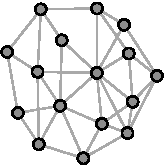
\includegraphics[width=.4\textwidth]{homophNet} & \hspace{2cm} &
	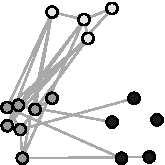
\includegraphics[width=.4\textwidth]{stochEquivNet}	
	\end{tabular}
	\caption{Graph on the left is a representation of an undirected network that exhibits a high degree of homophily, while on the left we show an undirected network that exhibits stochastic equivalence. }
	\label{fig:homphStochEquivNet}
\end{figure}

% How do different latent variable models compare? What structures do they represent? Homophily : similar nodes link to each other. ``similar'' may be in terms of unobserved characteristics. homophily leads to transitive or clustered social networks. observed transitivity may be due to exogenous or endogenous factors. stochastic equivalence: similar nodes have similar relational patterns. similar nodes may or may not link to each other. equivalent nodes can be thought of as having the same role. 

Another dependence pattern that cannot be accounted for in the framework discussed above is stochastic equivalence. A pair of actors $ij$ are stochastically equivalent if the probability of $i$ relating to, and being related to, by every other actor is the same as the probability for $j$ \citep{anderson:etal:1992}. More simply put this refers to the idea that there will be groups of nodes in a network with similar relational patterns. The occurrence of a dependence pattern such as this is not uncommon in an IR context. \citet{manger:etal:2012} theorize and estimate a stochastic equivalence structure to explain the formation of preferential trade agreements (PTAs). Specifically, they begin by dividing up countries into high, middle, and low income groups. They find that PTA formation occurs with greater probability in the following order high-middle, high-high, and middle-middle income groups, and that low income countries are rather unlikely to form PTAs with any partner. Such a structure is represented in the right-most panel of Figure~\ref{fig:homphStochEquivNet}, here the lightly shaded group of nodes at the top can represent high-income countries, nodes on the bottom-left middle-income, and the darkest shade of nodes low-income countries. The point here is just that the behavior of actors in a network can at times be governed by group level dynamics rather than attributes specific to an actor, and failing to account for patterns such as this could lead to discounting an important part of the data generating process. 

If we are able to account for the variety of shared attributes that might cause third order dependence patterns to develop then the additive effects described above is likely enough to justify our assumption of conditional independence and we can proceed to interpret our results. The \pkg{amen} package even provides for the estimation of that type of model using a Bayesian framework.\footnote{The main function in the \pkg{amen} package is titled ``ame'' and by default it runs a model assuming that no multiplicative effects are necessary. There are also a set of utilities one can use to determine whether the inclusion of multiplicative effects is necessary, we will review these in the following section.} In the context of most observational research, however, this assumption is untenable. The implausibility of an assumption such as this is, in spirit, the same reason why we no longer model time-series cross-sectional data without including, for example, country level fixed or random effects.

As \citet{cranmer:etal:2016} note a number of solutions have been suggested to this problem. They provide brief descriptions of the MRQAP and ERGM that we will not rehash here. The only point that we would emphasize from their discussion is that ERGMs should only be used when researchers are not only interested in modeling the specific set of third order patterns that may have given rise to a certain network, but also able to provide a theoretical justification for why those endogenous dependencies were specified over others. Failure to properly account for higher order dependence structures through an appropriate specification can at best lead to model degeneracy, which provides an obvious indication that the specification needs to be altered, and at worst a result that converges but does not appropriately capture the interdependencies in the network \citep{handcock:2003b,hunter:etal:2012}.\footnote{For a related discussion on the questionable tractability and consistency of modeling relational data through ERGMs see \citet{bhamidi:etal:2008,chatterjee:diaconis:2013,chandrasekhar:jackson:2014}.} The consequence of the latter case is a set of inferences that will continue to be biased as a result of unmeasured heterogeneity, thus defeating what we see to be a major motivation for pursuing an inferential network model in the first place. 

% The model can become degenerate, or place most of its probability on a few, disparate graphs, none of which resemble the observed network. A large amount of research has been devoted to iden- tifying the cause of this behavior (Bhamidi et al., 2008; Handcock, 2003a; Park and Newman, 2004, 2005), recognizing when it has occurred (Schweinberger, 2011; Hunter et al., 2008a), , and proposing modifications to the ERGM to avoid the issue (Snijders et al., 2006; Robins et al., 2007; Hunter, 2007). One hypothesized cause of the behavior are large and growing neigh- borhoods (Schweinberger and Handcock, 2012; Pattison and Robins, 2002), which lead to the local dependence dominating the global structure.

% describe local network structure, and by local network structure we mean features of nodes, we want to identify important nodes, groups of nodes and groups of nodes that are stochastically equivalent to each other (that is they have similar roles as one another), want to identify high density clusters (groups of nodes that have lots of ties to another). these are all features of particular nodes. 

% global network structures: how do explanatory variables relate to the socila network. how does the prevalence of ties relate to the presence of certain explantory varibales. might also be intersted in global measures like density and transitivity. 

Of more relevance to us in this paper is the review that \citet{cranmer:etal:2016} provide of latent space approaches. Of more relevance to us in this paper is the review that \citet{cranmer:etal:2016} provide of latent space approaches. Generally, the utilization of latent variable models for network analysis is a popular approach for modeling relational data in fields as diverse as computer science to the social sciences. One obvious reason for their continued usage is that they enable us to capture and visualize third order dependencies in a way that other approaches are not able to replicate. Additionally, the conditional independence assumption that these models are able to provide implies that model degeneracy is not an issue, facilitating the testing of a variety of nodal and dyadic level theories, and providing a range of computational advantages \citep{hunter:etal:2012}. 

They focus primarily on an approach that addresses third order dependency structures through embedding a graph onto a latent k-dimensional Euclidean space where the probability of a tie between nodes is decreasing in their distance in that space (we refer to this as the latent distance model). This approach was developed by \citet{hoff:etal:2002}, but, to our knowledge, the dominant approach in political science has been the latent factor approach, also known as the GBME, developed by \citet{hoff:2005} and introduced to political science by \citet{hoff:ward:2004}.\footnote{The latent factor approach is what has been used in: \citet{ward:etal:2007,cao:ward:2014,metternich:etal:2015}.} The distinction between these approaches is consequential and also informs the choices that were made in the creation of the alternative approach, AMEN, that we are introducing here.\footnote{There is one other major latent variable approach that we will leave undiscussed here referred to as the latent class model, or stochastic block model. In this model, nodes are assumed to belong to an unobserved latent class and a probability distribution is used to describe the relationships between classes \citep{nowicki:snijders:2001}. The probability of a tie between a pair of actors is a function of the classes to which they have been assigned. This type of model is useful as a community detection tool and is well suited for networks that exhibit high degrees of stochastic equivalence.} 

% \citet{krivitsky:handcock:2008} % \citet{krivitsky:handcock:2015} % implementation of latent space models % 

In the latent distance model, each node $i$ has some unknown latent position in $k$ dimensional space, $u_{i} \in R^{k}$, and the probability of a tie between a pair $ij$ is a function of the negative Euclidean distance between them: $-|u_{i}$ and $u_{j}|$. The basis 

The closer two actors are in this latent Euclidean space, the more likely they are to form an edge. This low-dimensional space can be thought of as a characteristic space where the distance between actors represents how similar they are (Hoff, Raftery, and Handcock 2002), or as a social space where the distance between two actors corresponds to the strength of the relationship between the two.

Because latent distances for a triple of actors must obey the triangle inequality, this formulation models the tendencies toward transitivity commonly found in social networks. A latent cluster model (Handcock, Raftery, and Tantrum 2007) is a variation on (10), specifying that latent positions for individual actors are mixtures of patterns associated with two or more latent categorical groups of actors. The LatentNet package in R (Handcock et al. 2007) uses Bayesian methods to fit such models.

Nodes nearby one another are more likely to have a tie and will likely have similar ties to others. One of the characteristics of this model is that if nodes are nearby one another they are highly likely to have a tie. But also if the nodes are closer together then they are going to be close to the same other nodes. So if you have two nodes that interact they are also similar form the perspective of other nodes. 

% this confounds the within tie density with stochastic equivalence. the model is going to do is try to put people who have ties to each other in the same location in space. characteristics of this model are a bit funny, in this model nodes that are nearby one another that means i and j have a tie, distnace between them is small, but also if i and j are very close to each other then the distance between i to k and j to k is going to be the same. so nodes that are very close to each other ar every likely to have a tie and likely to be stochastically equivalent. so this model confounds two patterns that we see in networks. 

% This pattern implies that vertices can be clustered by their latent positions. It then is natural to define a hierarchical model that explicitly represents such clusters within the latent space model [10]. But, homophily can be a misleading assumption for many real networks, which sometimes exhibit ordered (status-oriented) or disassortative patterns (dislike connects with dislike)

% \citet{hoff:2008} % critique of lat space eucl

% introduce via matrix decomposition, make a footnote to de finetti

% one final model is the latent factor model. this is an exchangeable random effects model. probability of a tie based ont he k dim space, btu the probability of the tie btween the two is going to depend on the inner and product of i and j's latent vector, weighted by some egien value. unlike the distance model, nodes iwth similar factors can have a large or small probability of tie. in the distance model if two things had the same value of i, the model wanted them to have a high probability of a tie. so in other words we can have negative eigen values. so if the bs are negative you could have it so that if things that are very similar to one another are unlikely to have a tie. here we can separate out: similar factors will be approximately stoch equiv, but unlike the dist model you dont have a confouding between high prob of ties and noedes having similar roles. Each node $i$ has an unknown latent factor. The probability of a tie from i to j depends upon their latent factors. This looks like an eigen decomposition of a latent matrix. Nodes with similar factors may have a large or small probability of a tie depdening on whether you have positive or negative eigen values. modes iwth similar facotrs are approximately stochastically equivalent. 

In sum, additive effects can capture network covariance. Multiplicative effects can capture higher-order dependence. 

\begin{align}
\begin{aligned}
	y_{ij} &= g(\theta_{ij}) \\ 
	&z_{ij} = \beta^{T} \mathbf{X}_{ij} + e_{ij} \\
	&e_{ij} = a_{i} + b_{j} + \epsilon_{ij} \\
	&\epsilon_{ij} = \gamma(u_{i}, u_{j}) + \mathcal{E}_{ij} \\
\end{aligned}
\end{align}

%%%%%%%%%%%%%%%%%%%%%%%%%%%
% de finetti's theorem will provide the basic tool and concept to generate a good statistical model. probability of obtaining one vector of random variables is the same as seeing that same vector permuted. if this condition holds for your probability model then you can describe these random variables as being equal to some global function theta, common to all random variables, and some variable specific random variable epsilon, wehere epsilon is iid from some probbaility distribution. 

% say we have a simple case where capital y is some symmetric binary matrix and we hav eno explanatory variables. and we have no information distinguishing nodes. say that you have some probabiltiy model that describes the network. yb = ya where nodes are relabeled. if we are treating ondes as unlabeled, then any probability model should set the probability of yb to be eqaul to ya. this property has a name and it is called row and column exchangeability. a probability model is row and coumn exchangeable if a given outcome little y is equal to another with nodes permuted. 

% if we have a rce array, then we can decompose our uncertaininty abotu thta random variable into some global parameter theta, some node specific effects, and some dyad specific effects. this isbasically saying that we should be looking at random effect models for models of social networks. so the question is what form shoul the g take from the slides. 

% Let $Y_{1} \ldots Y_{n}$ be an exchangeable sequence for all n:

% \begin{align}
	% Pr(Y_{1} = y_{1}, \ldots , Y_{n} = y_{n}) &= Pr(Y_{1} = y_{\pi_{1}}, \ldots , Y_{n} = y_{\pi_{n}}) \forall n
% \end{align}

% de Finetti's theorem says: 
% \begin{align}
% \begin{aligned}
	% Y_{i} &= g(\mu, \epsilon_{i}) \\
	% \epsilon_{1}, \ldots, \epsilon_{n} &\simiid p_{\epsilon}
% \end{aligned}
% \end{align}

% parameter $\mu$ represents global features of the sequence

% $\epsilon_{i}$ represents local features specific to individual $Y_{i}$

% This theorem justifies the ubiquitous conditional iid assumption of statistical modeling
%%%%%%%%%%%%%%%%%%%%%%%%%%%

%%%%%%%%%%%%%%%%%%%%%%%%%%%
%  stochastic blockmodel notes
% first latent variable mode is the latent class model (stochastic block model): each node i is a member of some unknown latent class, labeled 1 up to k. and each node is a member of some class. the probability of a tie between i and j is a function purely of their latent class, probability of a tie between any member of class 1 and class 2 is a functio of their class. interesting thing about this model is that the rate of ties from a member of class k to another member of class k is pheta kk, this may be a large number or small, number, the point is that members of the same class do not have to have a lot of ties to each other. have low density of common ties but they have common roles. and more generalyl nodes in the same class are stochastically equivalent, the probablity distribution for the relations that node i has is the same as the relations that node j has if i and j are in the same class. Each node $i$ is a member of an unknown latent class. $u_{i} \in (1,\ldots,K)$. The probability of a tie between i and j is only dependent upon the claseses. Nodes in the same class may have a small or high probability of ties. 
%%%%%%%%%%%%%%%%%%%%%%%%%%%